\label{sec:amyloid}
% A paragraph as a general introduction to amyloid.
% What's the general interest behind amyloid science -- why is amyloid important
% Role of amyloid in the human body -- functional amyloid?

Amyloids were discovered 150 years ago when tissue deposits of extracellular filaments were observed.\cite{Haass:2007db,Sipe:2000fs} These microscopically visible deposits were found on various organs in many seemingly unrelated diseases. 
%\textbf{Something should go here}
Although numerous diseases involve amyloid formation of distinct aggregation-prone proteins or peptides, the ability to form amyloid is not only restricted to these disease-associated proteins. Amyloid fibrils may be formed from proteins that can also fold into well-defined tertiary structures (e.g. myoglobin and lysozyme), suggesting that the ability to form amyloid fibrils may be a generic property of polypeptides.\cite{Chiti:2006fz} However, the propensity for a given protein or peptide to form amyloid fibrils is highly dependent on the combination of solution conditions and peptide sequence. This is because, for a globular protein to adopt amyloid states, the protein must first be partly unfolded before conversion into amyloid fibrils is possible.\cite{Chiti:2006fz} 
% TODO: Give a more specific example

% Dobson 2006 -- The relative aggregation rates for a wide range of peptides and proteins correlates with the physicochemical features of the molecules such as charge, secondary-structure propensities and hydrophobicity. 

% The mechanism of amyloid fibril formation \textit{in vivo} is not understood. However, \textit{in vitro} studies of amyloid-forming peptides in recent years have made great strides in elucidating their structural properties and mechanism of formation.
The pathway by which amyloid fibrils are formed \textit{in vivo} is not understood. Much of what we know about amyloid formation currently comes from biochemical and biophysical analysis of synthetic amyloid-forming peptides \textit{in vitro}, which is thought to be analogous to the \textit{in vivo} pathway. Prior to the appearance of amyloid fibrils, a variety of intermediate species may be formed.\cite{Chiti:2006fz} Monomers self-assemble into oligomers of different morphologies and sizes, which exist in equilibrium with amyloid fibrils, a visible endpoint of aggregation.\cite{Chiti:2006fz}

% Amyloid formation -- models of the kinetics of aggregation
Kinetically, the mechanism of amyloid formation is akin to those of nucleation-polymerization processes such as crystallization and micelle formation.\cite{Murphy:2002fe}
% \textbf{SPECIFIC CRYSTALLIZATION; SPECIFIC FORMATION OF OTHER PROTEINS FOLLOWING THIS PROCESS eg micelle formation} 
During nucleation, a lag phase occurs in which the energetic barriers of aggregation must be overcome by the monomers to form the initial aggregation nucleus.\cite{Murphy:2002fe} Following this lag phase, free monomers may bind to the nucleated aggregates, which elongate into mature fibrils.\cite{Murphy:2002fe} Seeding, a process where preformed aggregates are introduced into the solution, eliminates the lag phase.\cite{Harper:1997ix,Jarrett:1993vm} In the following sections, the current biophysical and structural data on amyloid fibrils and non-fibrillar oligomers is reviewed, and implications for amyloid disease are discussed.

% Because much of the detailed biochemical and biophysical characterization of amyloid formation is centered upon the amyloid-beta peptide (implicated in Alzheimer's disease) and hence our discussion will be focused on this peptide. % REWORD

% Focus mostly on biophysical data (it makes sense)
\subsection{Fibrils}

Fibrillar amyloid deposits have several physical properties in common. Fibrils are protease resistant, and insoluble in the presence of the detergent sodium dodecyl sulfate.\cite{Eisenberg:2012hm} Importantly, they exhibit specific optical behavior when bound to certain dye molecules. After staining with Congo red, fibrils exhibit bright green birefringence under polarized light.\cite{Frid:2007bo} However, the use of Congo red to detect the presence of amyloid formation is often a laborious process, and only provides a qualitative measurement of the amount of amyloid present.\cite{Frid:2007bo} Thioflavin-T (ThT), a benzathiole fluorescent dye, is more commonly used to detect the presence of amyloid fibrils in post-mortem brain tissue samples, and to monitor fibril formation \textit{in vitro}. Upon binding to fibrils, ThT exhibits both a dramatic enhancement of its emission and a shift in the maximum of its excitation spectrum, making it a sensitive and efficient reporter for the presence of amyloid fibrils.\cite{Nilsson:2004iw}

\begin{figure}
 \centering
 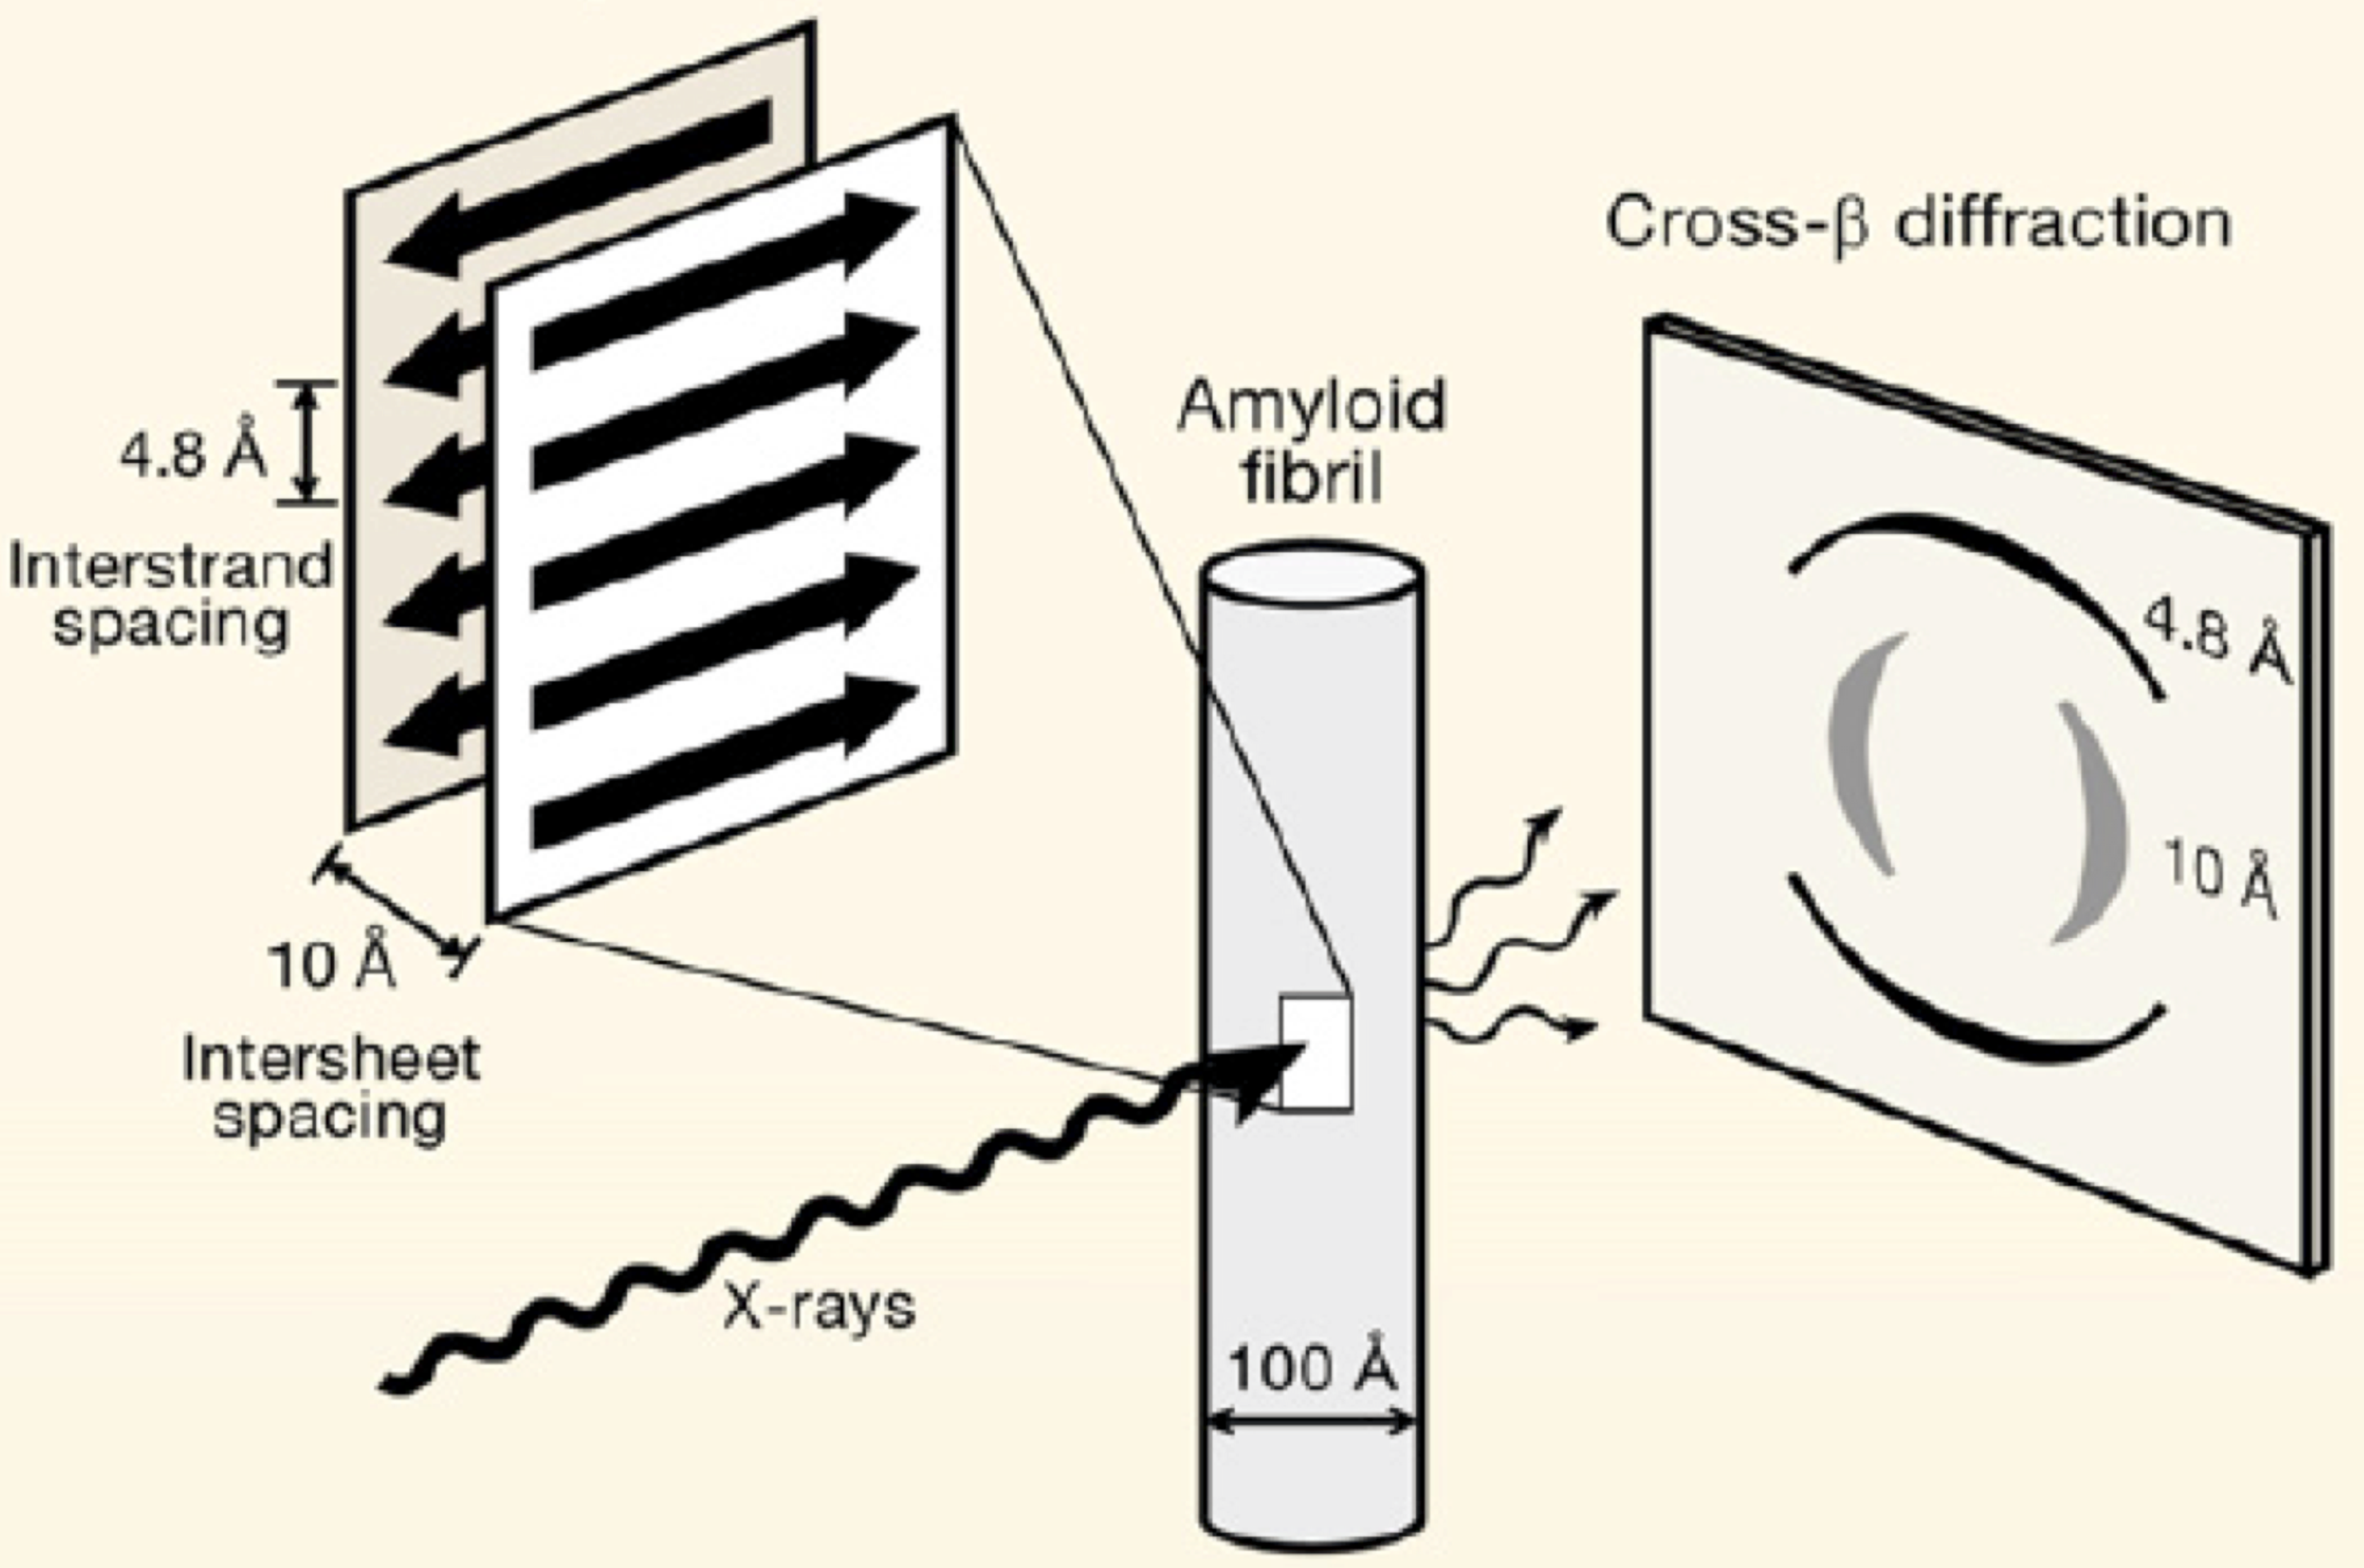
\includegraphics[width=5in]{figures/introduction/fibril_structure_diffraction.pdf}
 \caption[Characteristic cross-$\beta$ spacings from X-ray fibre diffraction studies of amyloid fibrils]{A schematic of the \crossbs\ and the diffraction pattern of fibrils. Reprinted from Cell, 148, D. Eisenberg, M. Jucker, The Amyloid State of Proteins in Human Diseases, 1188 - 1203., Copyright 2012, with permission from Elsevier.}
 \label{fig:fibril_diffraction}
\end{figure}

Amyloid fibrils formed from different polypeptides are thought to share a similar morphology known as the \crossbs.\cite{Chiti:2006fz} To date, independent measurements of fibrillar structure from different instruments have all confirmed the cross-$\beta$ structural core of amyloid fibrils. X-ray fiber diffraction studies showed that the diffraction pattern of fibrils is characterized by major orthogonal reflections along the meridional and equatorial directions, which correspond to a 4.8 \angstrom\ interpeptide separation, and a 10 \angstrom\ intersheet separation, respectively (Figure~\ref{fig:fibril_diffraction}).\cite{Sunde:1997cq,Makin:2005un,Sipe:2000fs} The inter-peptide and inter-sheet separations are respectively parallel and perpendicular to the long-axis of the fibril. This diffraction pattern is now considered as indicative of the presence of \crossbs, and hence, of amyloid fibrils.\cite{Chiti:2006fz} When the fibrils are stained the macromolecular morphology of fibrils can be determined using the transmission electron microscope (TEM): fibrillar structures are long, unbranched, and ribbon-like structures with diameters between 50 - 100 nm (Figure~\ref{fig:fibril_TEM_SSNMR}).\cite{Chiti:2006fz} 
% Other measurements? - MPL Mass per unit length?

% Although \crossb\ is widely known, due to the insolubility and inherent non-crystalline nature of amyloid fibrils, the molecular details of the fibril structure remained elusive until recent years. 
% The ubiquitous presence of a \crossbs\ supports that the organization of the peptidic backbone, common to all proteins, in to \bsheets\ is a major determinant of the fibrillar structure. 

\begin{figure}
 \centering
 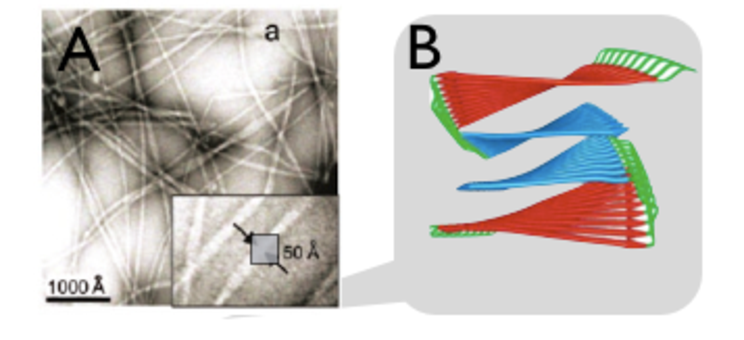
\includegraphics[width=4in]{figures/introduction/fibril_TEM_SSNMR.pdf}
 \caption[EM images of amyloid fibrils and oligomers]{(A) TEM image of negatively-stained mature amyloid fibrils.\cite{Petkova:2002p305} Copyright 2002 National Academy of Sciences, USA. (B) SSNMR model proposed by Tycko et al. Reprinted (adapted) with permission from\cite{Petkova:2006gx}. Copyright 2006 American Chemical Society. EM images of oligomers of (C) \abeta42,\cite{Bitan:2003ut} and (D) \abeta40. (C) Copyright 2003 National Academy of Sciences, USA. (D) This research was originally published in Journal of Biological Chemistry. D M Walsh, D M Hartley, Y Kusumoto, Y Fezoui, M M Condron, A Lomakin, G B Benedek, D J Selkoe, and D B Teplow. Amyloid $\beta$-Protein Fibrillogenesis. Journal of Biological Chemistry. 1999; 274:25945-25952. \copyright\ the American Society for Biochemistry and Molecular Biology.}
 \label{fig:fibril_TEM_SSNMR}
\end{figure}

\begin{figure}
 \centering
 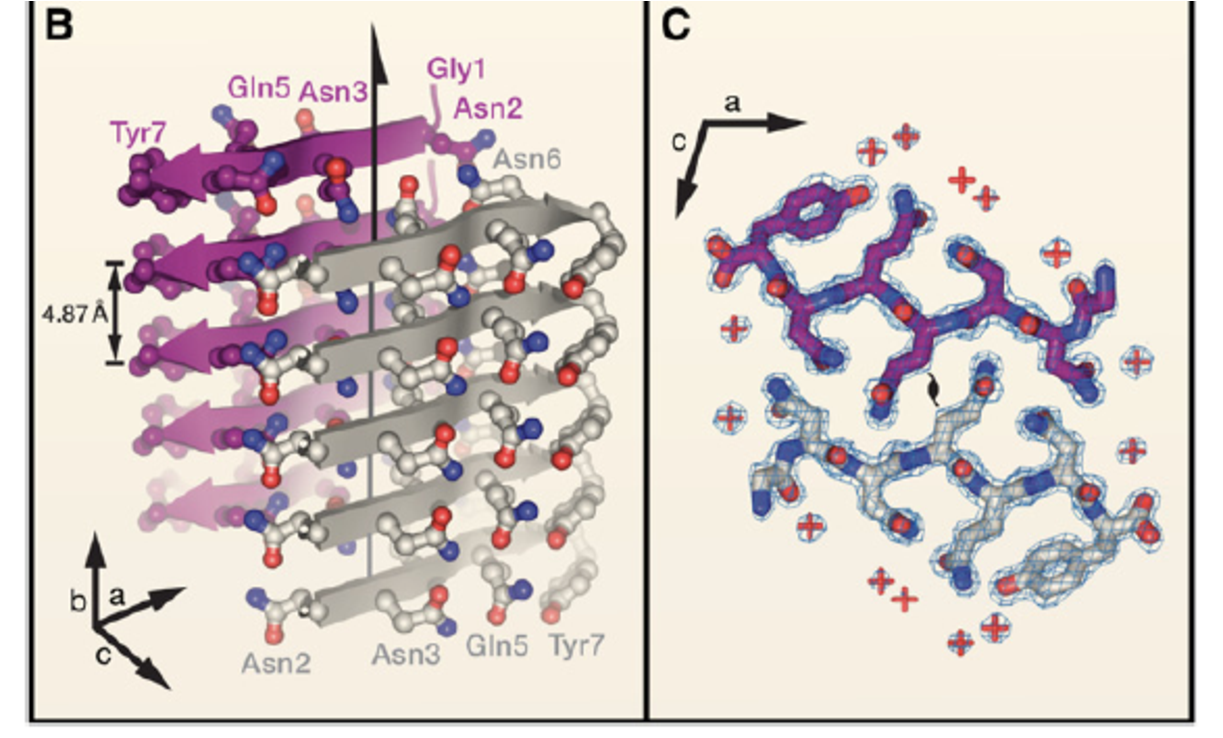
\includegraphics[width=4in]{figures/introduction/fibril_xray_model.pdf}
 \caption[X-ray crystal structure of an amyloid fibril]{A schematic of the X-ray crystal structure of fibrils formed from short amyloidogenic peptide fragments. Reprinted from Cell, 148, D. Eisenberg, M. Jucker, The Amyloid State of Proteins in Human Diseases, 1188 - 1203., Copyright 2012, with permission from Elsevier.}
 \label{fig:fibril_xray_model}
\end{figure}

% Describe the molecular structure of \abeta\ amyloid fibrils. Briefly mention the techniques that can be used to obtain structural information of amyloid fibrils. 

% SSNMR
Advances in solid-state NMR (SSNMR) and X-ray crystallography in the last decade have elucidated the molecular details of amyloid fibrils. One of the first SSNMR models of an amyloid fibril was that of \textbf{\abeta40}, a peptide implicated in Alzheimer's Disease.\cite{Petkova:2006gx}
%The study by Petkova et. al.\cite{Petkova:2006gx} indicated that the \bsheet\ core of \abeta40\ involves residues 10-22 and 30-40, and is linked by a loop formed by residues 23-29. 
Its core fibril unit consists of a parallel in-register \bsheet, where each strand is a \bhairpin\ with peptide-peptide backbone hydrogen bonds running parallel to the long-axis of the fibril (Figure~\ref{fig:fibril_TEM_SSNMR}). Moreover, smaller fragments of A$\beta$ have been shown to form fibrils that are morphologically similar to those of the full length peptide. For example, SSNMR studies of the fibrils of the peptide A$\beta$(16-22), the central hydrophobic core of A$\beta$, with sequence KLVFFAE, indicated that its fibrils are composed of stacked antiparallel $\beta$-sheets.\cite{Balbach:2000vf} Furthermore, fibrils of certain amyloid-forming peptide fragments formed crystals that were amenable to single crystal X-ray diffraction analysis.\cite{Eisenberg:2012hm} In agreement with SSNMR, the crystal structures of these fibrils revealed a structure composed of multiple layers of \bsheet\ with a dehydrated (``dry'') stacking interface (Figure~\ref{fig:fibril_xray_model}).\cite{Sawaya:2007p4363,Eisenberg:2012hm}
%Taken together, these recently proposed structures demonstrate that the core region is composed of two to four sheets that interact closely with each other. % I don't think I will talk about the twisting of the sheets too much. Should I mention twisting?

% Fibril polymorphism
The particular packing arrangement of polypeptides in amyloid fibrils can vary with changes in the experimental conditions under which the fibrils are formed. Specific structural polymorphisms include the length of the $\beta$-strands, side chain orientations and inter-protofilament packing.\cite{Kodali:2007cz} Fibril polymorphism may have important implications in amyloid diseases because different morphologies exhibit differing toxicities that depend on which residues are exposed at the surface. For example, \textit{in vitro}, quiescently formed fibrils of A$\beta$(1-40) have been shown to be more toxic than agitated fibrils.\cite{Petkova:2005p4688} 

% A polymorphic structure introduced by a seed have been shown to be able to propagate \textit{in vitro}.\cite{Paravastu:2006p4690} A recent study propagated a brain-derived fibril fragment in order to obtain structural information on fibrils that most closely resembles those formed in the AD brain.\cite{Paravastu:2009fi} -- These points aren't going anywhere.

% http://onlinelibrary.wiley.com/doi/10.1111/j.1742-4658.2010.07888.x/abstract?systemMessage=Wiley+Online+Library+will+be+disrupted+on+15+December+from+10%3A00-12%3A00+GMT+%2805%3A00-07%3A00+EST%29+for+essential+maintenance

\subsection{Non-fibrillar oligomers}

Because of their structural disorder and transient nature, it is difficult to obtain high-resolution structural details of amyloid oligomers using traditional structural determination techniques. Studies using low-resolution techniques transmission electron microscopy (TEM) and atomic force microscopy (AFM) have shown that transient, unstable particles may appear prior to the formation of fibrils (``on-pathway'' oligomers).\cite{Chromy:2003p2575,Ahmed:2010p5694,Caughey:2003jq} These protein aggregates are referred to in literature as amyloid protofibrils.\cite{Chiti:2006fz} Those that do not progress to form fibrils are considered off-pathway.\cite{Kayed:2003en} However, off-pathway oligomers formed in the presence of detergents, lipids, and certain small molecules are typically not considered to be biologically-relevant.\cite{Yu:2009p2873,Laurents:2005ki}
% Oligomers may either be on-pathway to fibril formation, that is, they serve only as intermediates, while others themselves may be the endpoints of aggregation.
% Currently, the precise mechanism involved in the transition from oligomers to extended amyloid fibrils is not known.

Unlike fibrils, amyloid oligomers do not possess a generic structural element and instead, adopt a wide spectrum of sizes and morphologies. Size exclusion chromatography (SEC) studies of \abeta40\ oligomers (isolated \textit{in vitro} and from the brains of deceased individuals with Alzheimer's Disease) revealed the existence of oligomers that ranged in size from dimers to large oligomers of hundreds of peptides.\cite{Haass:2007db,Walsh:2007fu} Oligomeric assemblies that are annular, spherical, or curvilinear in shape have been reported in literature.\cite{Haass:2007db,Kim:2009p2715,Lashuel:2002eg}

% This was directly copied from Fandrich 2012
Although there are large variations in morphologies, oligomers formed from different polypeptide sequences can display similar activities in cell metabolic assays.\cite{Bucciantini:2002un} Importantly, many oligomers of different sizes share the ability to interact with a single oligomer-specific antibody.\cite{Kayed:2003en,Glabe:2008p130} % Large spherical oligomers (3-10nm in diameter) formed from disparate sequences have been shown to binding to a single antibody, which suggests that they may share similar structural elements.
Several studies have indicated that oligomers may possess high $\beta$-sheet content.\cite{Walsh:1999up,Chimon:2007du,Ahmed:2010p5694,Campioni:2010hz} % also bind dyes Thioflavin T (ThT) and Congo Red (CR).\cite{Walsh:2007fu,Haass:2007db,Kodali:2007cz}
Moreover, some non-fibrillar oligomers may contain common structural elements: high-resolution structural studies of non-fibrillar oligomers of \abeta42\ and prion-like peptides suggest that they may contain \crossb\ like fragments.\cite{Walsh:2010p4761,Stroud:2012dp,Chimon:2007du}
 % Should briefly read up on the book chapter by Pat Walsh and cite him
 
% Although oligomers particles may be \bsheet-rich, they are morphologically distinct from fibrils (Figure~\ref{fig:oligomers}).\cite{Walsh:2009p1235}. 
% And may contain random-coil-like conformations\cite{Sandberg:2010ix}

% References for the morphologies from Pat's thesis introd -- (Janson et al. 1999; Conway et al. 2000; Lashuel et al. 2002)
%Conway, K. A., Harper, J. D. and Lansbury, P. T., Jr. (2000). Fibrils formed \textit{in vitro} from alpha-synuclein and two mutant forms linked to Parkinson's disease are typical amyloid. Biochemistry, Vol. 39, No. 10, pp. 2552-63.
%Conway, K. A., Lee, S. J., Rochet, J. C., Ding, T. T., Williamson, R. E. and Lansbury, P. T., Jr. (2000). Acceleration of oligomerization, not fibrillization, is a shared property of both alpha-synuclein mutations linked to early-onset Parkinson's disease: implications for pathogenesis and therapy. Proceedings of the National Academy of Sciences of the United States of America, Vol. 97, No. 2, pp. 571-6.
%Janson, J., Ashley, R. H., Harrison, D., McIntyre, S. and Butler, P. C. (1999). The mechanism of islet amyloid polypeptide toxicity is membrane disruption by intermediate-sized toxic amyloid particles. Diabetes, Vol. 48, No. 3, pp. 491-8.

% Outline some of the ideas / hypothesis about the link between amyloid and disease, but don't go into what people speculate or data on toxicity. It is related, but this is out of the scope of your thesis.
% Although not the focus of this thesis, understanding the mechanism of toxicity and elucidating the underlying toxic species will be important in the development of future drug candidates.
%Papers talking about the links of oligomers to disease\cite{Lansbury:2006p928,Lashuel:2006co}